\documentclass[11pt,a4paper]{article}
\usepackage{fontspec}
\setmainfont{TeX Gyre Pagella}
\newfontfamily\headfont{Inter}[UprightFont=*-ExtraBold,BoldFont=*-ExtraBold,Extension=.otf,Path=/usr/share/fonts/opentype/inter/]
\usepackage[a4paper,margin=2.3cm]{geometry}
\usepackage{graphicx,booktabs,float,caption,array,xcolor,longtable}
\usepackage{xurl}
\usepackage[hidelinks]{hyperref}
\usepackage{titlesec}
\usepackage[round]{natbib}
\usepackage{setspace}
\setstretch{1.05}
\renewcommand{\topfraction}{0.9}
\renewcommand{\bottomfraction}{0.8}
\renewcommand{\textfraction}{0.1}
\renewcommand{\floatpagefraction}{0.75}
\setlength{\parindent}{0pt}
\setlength{\parskip}{0.55em}
\titleformat{\section}{\headfont\Large}{\thesection}{0.8em}{}
\titleformat{\subsection}{\headfont\large}{\thesubsection}{0.8em}{}
\captionsetup{font=small,labelfont=bf}
\urlstyle{same}
\hypersetup{pdftitle={Fighting by Moonlight},pdfauthor={Tristan Hotham}}


\begin{document}
\begin{center}
{\Large\bfseries Fighting by Moonlight\par}
\vspace{0.4em}
{\large The phase of the Moon on the days of 9,877 dated battles, with a calendar-aware null\par}
\vspace{1.2em}
{\large Tristan Hotham\par}
\vspace{0.3em}
{\small Independent researcher\\
ORCID: 0000-0003-4931-9349\\
DOI: https://doi.org/10.5281/zenodo.24089704\par}
\vspace{0.8em}
2026
\end{center}

\begin{quote}
\small
\begin{center}\textbf{Abstract}\end{center}
Commanders have long timed night marches, landings and dawn attacks by the Moon, but whether the Moon shaped the dates of battles in general has not been measured. I compute the Moon's phase on the day, and the Sun and Moon through the night before, at the site of every battle in Wikidata with a day-precision date and coordinates, 9,877 battles from AD 69 to 2026 after calendar checks. Wikidata stores dates converted to the proleptic Gregorian calendar with a flag for the calendar of entry; I show that pre-1582 dates flagged Gregorian are almost always Julian dates, correct 346 of them, check British Old Style dates before 1752 by hand or exclude them, and confirm 21 of 21 famous dates against the standard histories and four against recorded eclipses or lunar calendars. Against a null of random days from each battle's own century, simulated 2,000 times, the eight-phase distribution does not differ from chance ($p=0.20$). There is a faint lean towards the bright half of the month: mean illuminated fraction 51.1\% against 50.0\% (Rayleigh $p=0.016$, mean direction 182\textdegree), equivalent to about 2\% of battles timed for a full Moon, which is not robust to counting one battle per date ($p=0.054$) or to keeping only battles with their own coordinates ($p=0.16$). No era, from the medieval to the post-1945, shows a significant pattern. Against season-matched random nights, the Moon was up for 6 minutes more of the darkness before battles, and no more often at dawn. The Moon is a famous factor in particular operations, such as the Normandy landings, but not a general driver of when battles were fought.

\textbf{Keywords:} lunar phase; battles; military history; Wikidata; calendar conversion; circular statistics; astronomy
\end{quote}

\section{Introduction}
The Moon has a reputation in warfare. The Normandy landings of June 1944 were set for a Moon near full, for the airborne drops, and a low but rising tide soon after dawn; bomber crews spoke of a ``bomber's Moon''; the Second Battle of El Alamein opened at night under a bright Moon. Ancient historians recorded eclipses on the eves of battles \citep{livy,herodotus}. But anecdotes select themselves. This paper asks a simpler, general question: across all battles with a known day and place, does the Moon's phase or the moonlight of the night before depart from what chance would give?

Two difficulties make this harder than it looks. First, calendars: a date entered in the Julian calendar but read as Gregorian, or the reverse, is shifted by up to ten days, a third of a lunar cycle. Second, the null: the phase of the Moon on random calendar days is not exactly uniform over short windows, and moonlight on a given night depends on the season and latitude as well as the phase, so a fair comparison must use random days from the same period and, for moonlight, the same place and season.

\section{Data}
\textbf{Battles.} Items that are instances of battle (Q178561) or its subclasses in Wikidata \citep{wikidata}, queried with QLever \citep{qlever}, with a point in time (P585) or start time (P580) at day precision, coordinates (P625) or the coordinates of their location (P276), the war they are part of, and their number of Wikipedia sitelinks. Sieges (Q188055 and subclasses), which last weeks, are kept apart. Of 13,747 items with day-precision dates, 1,452 have no coordinates; of the 12,295 with both, 2,021 are sieges and 10,274 battles. Where an item has several dates within three days I take the earliest (the first day of fighting); 183 battles with dates more than three days apart are excluded from the tests. 3,145 battles in the test are placed at the coordinates of their location. A battle is at sea if its point lies more than about 3 km from Natural Earth land (588 battles).

\textbf{Calendars.} In the Wikidata RDF export, time values are given in the proleptic Gregorian calendar and the calendar model records the calendar in which the date was entered (Q1985727 Gregorian, Q1985786 Julian). Checking famous battles confirms this: Hastings, entered as 14 October 1066 (Julian), is stored as 20 October; Pydna, 22 June 168 BC (Julian), as 19 June. Julian-flagged values are therefore used as stored. Gregorian-flagged values before 15 October 1582, when no source used the Gregorian calendar, are in case after case the usual Julian date with the wrong flag (Bosworth, 22 August 1485; Towton, 29 March 1461, Palm Sunday; Stamford Bridge, 25 September 1066; Mohács, 29 August 1526); I reinterpret all 346 as Julian. Britain, Ireland and British North America used the Julian (Old Style) calendar until September 1752; among their Gregorian-flagged dates before then, many English Civil War dates are Old Style (Naseby, 14 June 1645; Marston Moor, 2 July 1644) while others are correctly converted (Culloden, 27 April 1746). I settled 31 by hand (\texttt{code/overrides.csv}) and exclude the remaining 175 from the tests, with the 39 dates before AD 1, which rest on modern conversions of ancient calendars. One further date was corrected by hand: Kosovo, 1389, entered as 28 June with a Julian flag (stored as 6 July), but 28 June is the modern Gregorian date of St Vitus' Day, so the date has in effect been converted twice; I use 15 June 1389 (Julian). Calendar conversions follow standard algorithms \citep{reingold}. Table~\ref{tab:cal} lists the 21 hand checks; all agree.

\begin{table}[tbp]\centering\footnotesize\caption{Hand checks of the calendar handling: the date in the standard histories, the date the pipeline settles (Gregorian), the flag in Wikidata and the rule applied. For Bannockburn the pipeline gives the first of the two days.}\label{tab:cal}\begin{tabular}{llllr}\toprule Battle & Standard date & Pipeline (Gregorian) & Flag & Rule\\\midrule
Hastings & 14 October 1066 (Julian) & 20 October 1066 & J & julian\\
Agincourt & 25 October 1415 (Julian) & 3 November 1415 & J & julian\\
Crécy & 26 August 1346 (Julian) & 3 September 1346 & J & julian\\
Bosworth Field & 22 August 1485 (Julian) & 31 August 1485 & G & reflagged\\
Towton & 29 March 1461 (Julian) & 7 April 1461 & G & reflagged\\
Stamford Bridge & 25 September 1066 (Julian) & 1 October 1066 & G & reflagged\\
Bannockburn & 24 June 1314 (Julian) & 1 July 1314 & J & julian\\
Lepanto & 7 October 1571 (Julian) & 17 October 1571 & J & julian\\
Naseby & 14 June 1645 (Julian) & 24 June 1645 & G & os\_override\\
Marston Moor & 2 July 1644 (Julian) & 12 July 1644 & G & os\_override\\
Edgehill & 23 October 1642 (Julian) & 2 November 1642 & J & julian\\
the Boyne & 1 July 1690 (Julian) & 11 July 1690 & J & julian\\
Culloden & 16 April 1746 (Julian) & 27 April 1746 & G & os\_checked\\
Poltava & 27 June 1709 (Julian) & 8 July 1709 & J & julian\\
Blenheim & 13 August 1704 (Gregorian) & 13 August 1704 & G & gregorian\\
Waterloo & 18 June 1815 (Gregorian) & 18 June 1815 & G & gregorian\\
Borodino & 7 September 1812 (Gregorian) & 7 September 1812 & G & gregorian\\
Gettysburg & 1 July 1863 (Gregorian) & 1 July 1863 & G & gregorian\\
the Somme & 1 July 1916 (Gregorian) & 1 July 1916 & G & gregorian\\
Pydna & 22 June 168 BC (Julian) & 19 June 168 BC & J & ancient\\
Halys & 28 May 585 BC (Julian) & 22 May 585 BC & J & ancient\\
\bottomrule\end{tabular}\end{table}

\section{Method}
\textbf{The Moon.} For each battle, at its site, astronomy-engine \citep{astronomyengine} gives the Moon's phase angle (its elongation from the Sun in ecliptic longitude: 0\textdegree{} new, 90\textdegree{} first quarter, 180\textdegree{} full, 270\textdegree{} last quarter), its illuminated fraction and its age at local mean noon of the battle day, and the topocentric altitudes of the Sun and Moon, with standard refraction, every ten minutes from local noon of the day before to local noon of the battle day. Darkness is the Sun more than 6\textdegree{} below the horizon; the Moon is up when its upper limb is above the horizon. From these I take the hours of darkness, the hours of darkness with the Moon up, and whether the Moon was up at sunrise. An independent ephemeris, PyEphem \citep{pyephem}, agrees on the phase of every famous battle in Table~\ref{tab:famous} to within 0.3\textdegree.

\textbf{Null.} For phase, each battle gets 2,000 random days drawn uniformly from its own century, at its own longitude; the phase of each is computed with the mean lunar elements and the six largest periodic terms of the phase angle \citep{meeus}, which agree with astronomy-engine to a median of 0.12\textdegree{} (99th percentile 0.5\textdegree) on 98,770 test nights. Each of the 2,000 simulated data sets gives a null distribution for every statistic: the $\chi^2$ of eight equal phase bins against their simulated expectation, the Rayleigh resultant length $R$ of the phase angles and its second harmonic \citep{fisher1993}, the number of battles within 1.5 days of full Moon, and the mean illuminated fraction. The $p$-values are the share of simulated sets at least as extreme. For moonlight the null is ten random nights per battle at the same site, in a random year of the same century and within 15 days of the same date in the year; a first run with century-uniform dates showed that nights before battles are shorter than random nights, a summer bias that would otherwise pass for a moonlight effect; with season matching the hours of darkness agree (10.19 against 10.19).

\section{Results}
\subsection{Phase}
Table~\ref{tab:bins} and Figure~\ref{fig:wheel} give the battles in eight phase bins against the simulated expectation. The spread does not differ from chance ($\chi^2=9.9$, $p=0.20$). The Rayleigh test detects a small lean of the phase angles towards 182\textdegree, that is towards full Moon ($R=0.021$, $p=0.016$). In plainer terms, the Moon was on average 51.1\% lit on battle days against 50.0\% for random days, and 10.6\% of battles fell within 1.5 days of full Moon against 10.0\% expected (about 63 battles). If a share $f$ of battles had been timed for a fully lit Moon and the rest were random, the mean lit fraction would be $0.5 + 0.5f$: the observed difference corresponds to $f \approx 2.1\%$. There is no bimodality (second harmonic $p=0.95$): new and full Moon are not jointly favoured. A season-matched phase null gives the same result ($\chi^2$ $p=0.22$, Rayleigh $p=0.016$).

\begin{table}[tbp]\centering\small\caption{Battles by phase of the Moon (eight equal bins centred on the named phases) against the expectation from 2,000 simulated sets of random days.}\label{tab:bins}\begin{tabular}{lrrrr}\toprule Phase & Battles & Expected & Share (\%) & Ratio\\\midrule
New moon & 1,169 & 1,212.7 & 11.84 & 0.964\\
Waxing crescent & 1,189 & 1,230.9 & 12.04 & 0.966\\
First quarter & 1,224 & 1,256.1 & 12.39 & 0.974\\
Waxing gibbous & 1,280 & 1,237.5 & 12.96 & 1.034\\
Full moon & 1,274 & 1,216.4 & 12.90 & 1.047\\
Waning gibbous & 1,278 & 1,234.7 & 12.94 & 1.035\\
Last quarter & 1,248 & 1,254.2 & 12.64 & 0.995\\
Waning crescent & 1,215 & 1,234.5 & 12.30 & 0.984\\
\bottomrule\end{tabular}\end{table}

\begin{figure}[tbp]\centering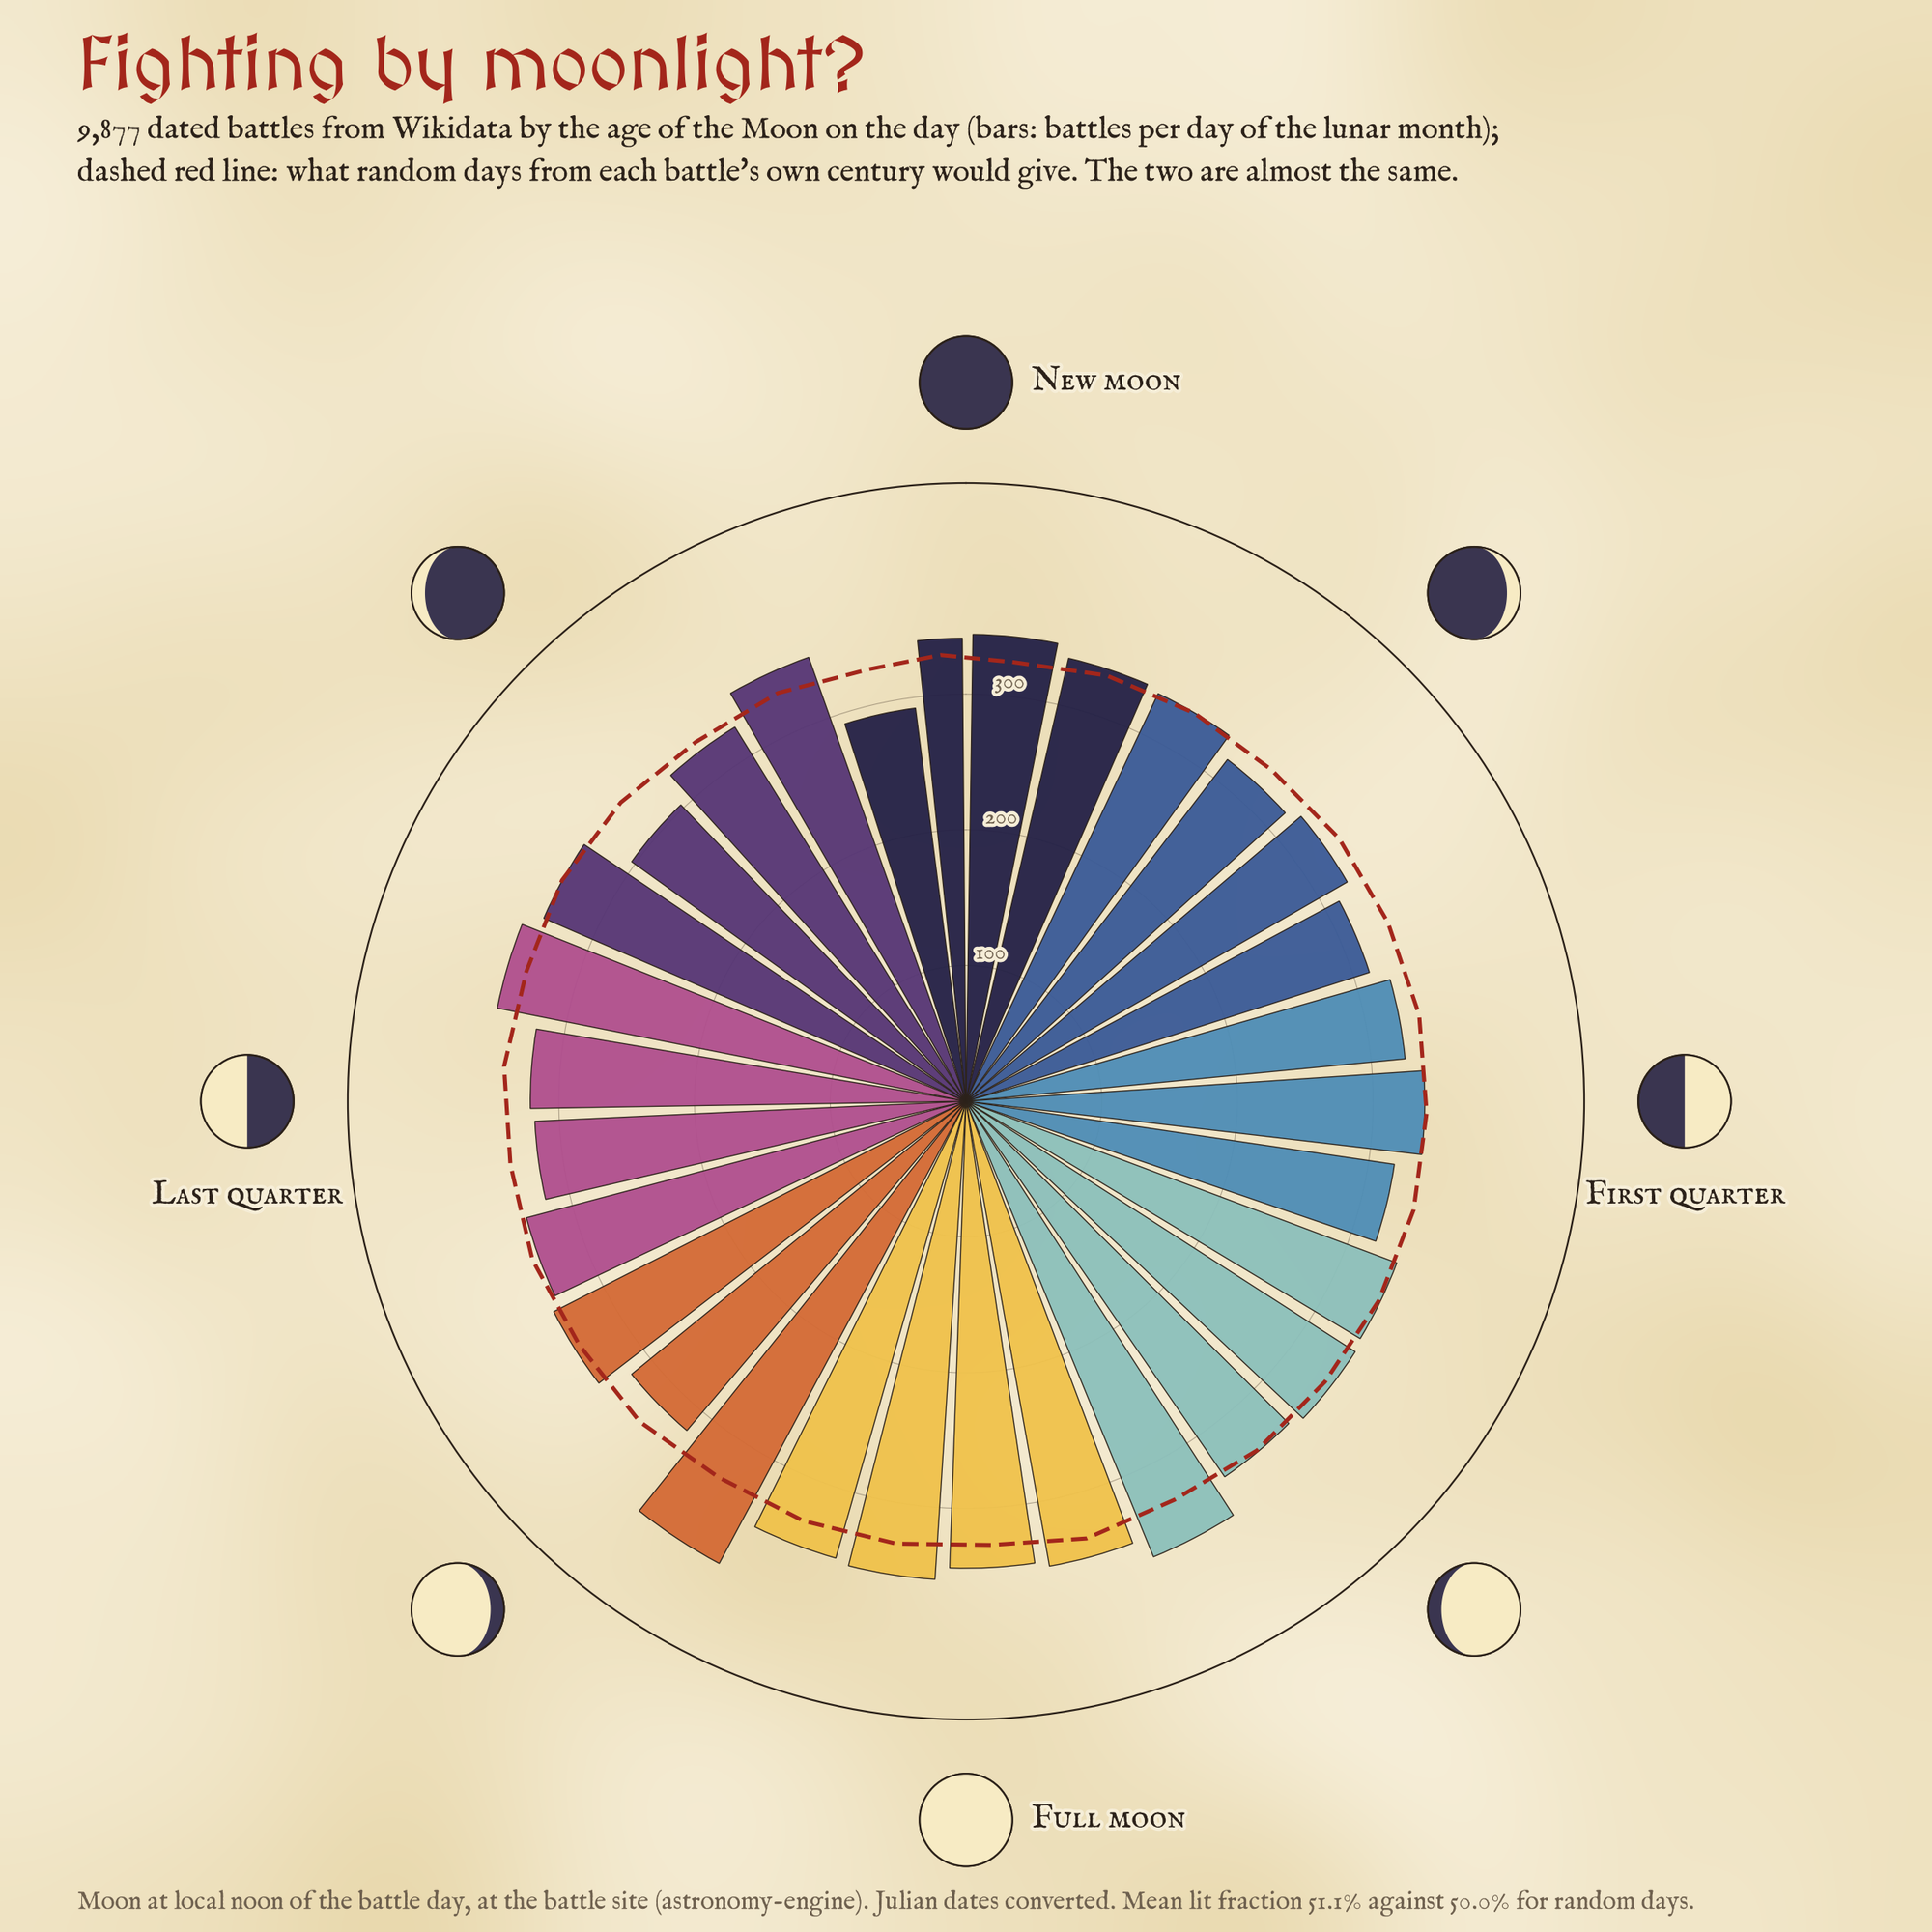
\includegraphics[width=0.82\textwidth]{f_wheel.png}
\caption{Battles per day of the lunar month (bars) against random days from each battle's century (dashed).}\label{fig:wheel}\end{figure}

\subsection{Robustness}
The lean is fragile (Table~\ref{tab:sens}). It survives leaving out the dates whose flag I corrected and adding the uncertain ones, but weakens when sub-battles on the same day are counted once ($p=0.054$), when only dates after the Gregorian reform are kept ($p=0.066$) and when only battles with their own coordinates are kept ($p=0.16$). With several groupings and tests reported, a single $p$ near 0.02 is weak evidence.

\begin{table}[tbp]\centering\footnotesize\caption{Sensitivity of the phase tests to the calendar rules and the data.}\label{tab:sens}\begin{tabular}{p{8.2cm}rrrr}\toprule Variant & $n$ & Lit (\%) & $\chi^2$ $p$ & Rayleigh $p$\\\midrule
All battles in the test & 9,877 & 51.1 & 0.20 & 0.016\\
Leaving out the pre-1582 dates whose flag I corrected & 9,581 & 51.1 & 0.22 & 0.011\\
Only dates after the Gregorian reform (from 15 October 1582) & 8,328 & 50.9 & 0.62 & 0.066\\
Adding the uncertain British Old Style dates and the ancient dates & 10,091 & 51.0 & 0.19 & 0.019\\
Leaving out dates on the 1st of a month (possible month-only dates) & 9,542 & 51.0 & 0.21 & 0.040\\
Only battles with their own coordinates & 6,732 & 50.9 & 0.56 & 0.163\\
One battle per date (sub-battles of the same day counted once) & 8,740 & 51.0 & 0.31 & 0.054\\
\bottomrule\end{tabular}\end{table}

\subsection{Eras and kinds of battle}
No era shows a phase pattern (Table~\ref{tab:groups}, Figure~\ref{fig:eras}). The Second World War comes closest: 136 of 930 battles in the full-Moon bin against 113.9 expected (Rayleigh $p=0.07$). Battles at sea (588), raids and ambushes named as such (71), the best-known battles (30 or more Wikipedia editions, 252) and sieges (1,876) show nothing (Figure~\ref{fig:groups}).

\begin{table}[tbp]\centering\footnotesize\caption{Tests by era and kind of battle: number, mean illuminated fraction (\%) against random days, share within 1.5 days of full Moon (\%), and simulated $p$ for the $\chi^2$ and Rayleigh tests (1,000 to 2,000 simulated sets).}\label{tab:groups}\begin{tabular}{lrrrrrr}\toprule Group & $n$ & Lit & Random & Near full & $\chi^2$ $p$ & Rayleigh $p$\\\midrule
Before 1500 & 1,127 & 52.1 & 50.0 & 10.9 & 0.25 & 0.139\\
1500 to 1799 & 2,525 & 50.5 & 50.0 & 10.0 & 0.78 & 0.380\\
1800 to 1899 & 2,867 & 51.2 & 50.0 & 10.0 & 0.43 & 0.225\\
1900 to 1945 & 2,009 & 50.7 & 50.1 & 11.7 & 0.17 & 0.560\\
1946 to 2026 & 1,349 & 51.7 & 50.1 & 11.3 & 0.49 & 0.128\\
On land & 9,289 & 51.2 & 50.1 & 10.7 & 0.10 & 0.005\\
At sea & 588 & 48.9 & 50.0 & 9.0 & 0.61 & 0.578\\
Raids, ambushes and surprise attacks & 71 & 45.7 & 49.9 & 9.9 & 0.09 & 0.118\\
First World War, 1914 to 1918 & 587 & 48.1 & 50.1 & 11.1 & 0.14 & 0.334\\
Second World War, 1939 to 1945 & 930 & 52.6 & 50.1 & 12.6 & 0.12 & 0.068\\
Well known (30 or more Wikipedia editions) & 252 & 50.8 & 50.0 & 7.9 & 0.07 & 0.746\\
Sieges (start date) & 1,876 & 49.1 & 50.0 & 8.9 & 0.35 & 0.441\\
\bottomrule\end{tabular}\end{table}

\begin{figure}[tbp]\centering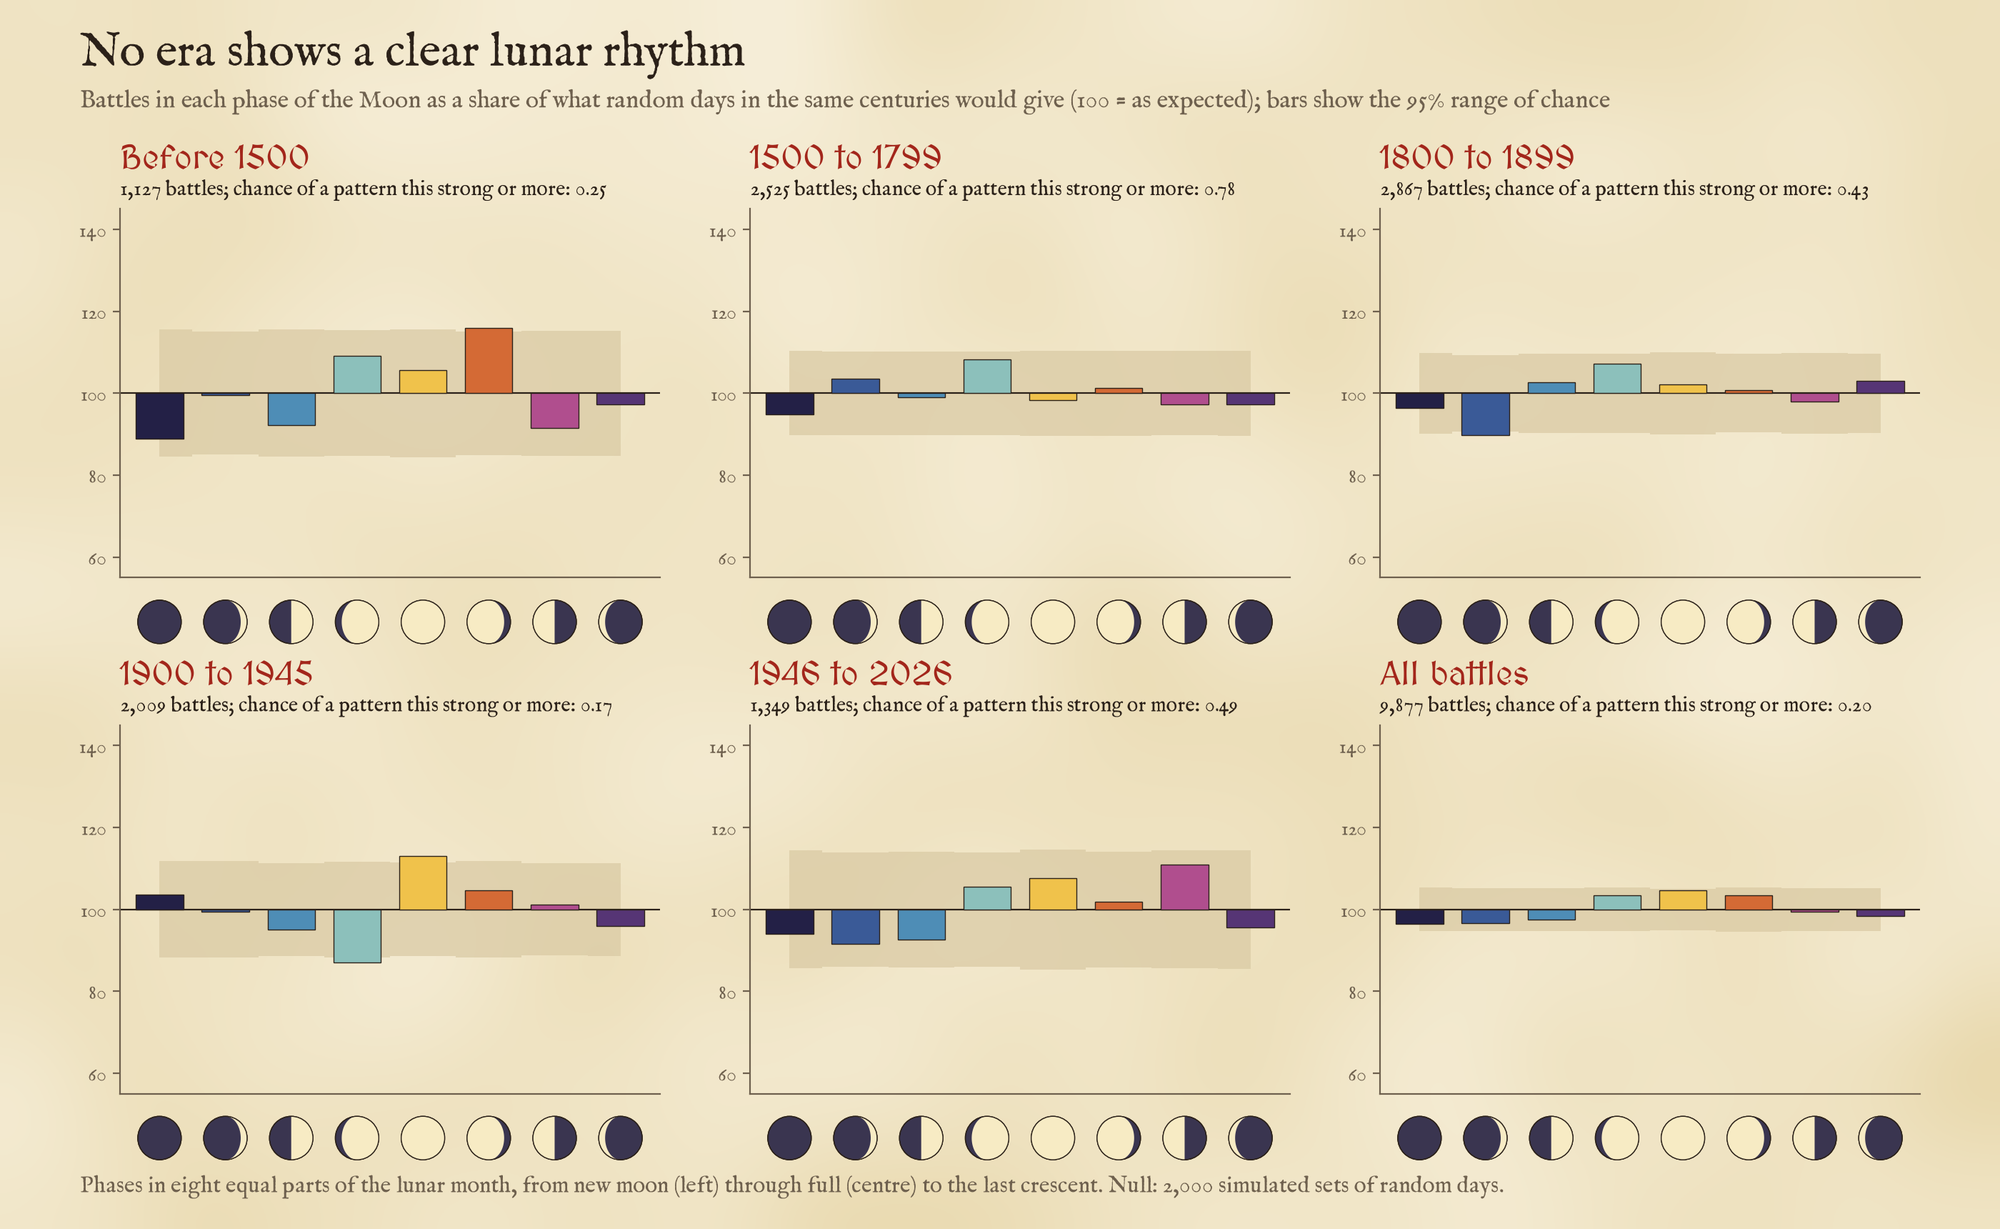
\includegraphics[width=\textwidth]{f_eras.png}
\caption{Battles in each phase bin as a share of the simulated expectation, by era, with the 95\% range of chance.}\label{fig:eras}\end{figure}

\begin{figure}[tbp]\centering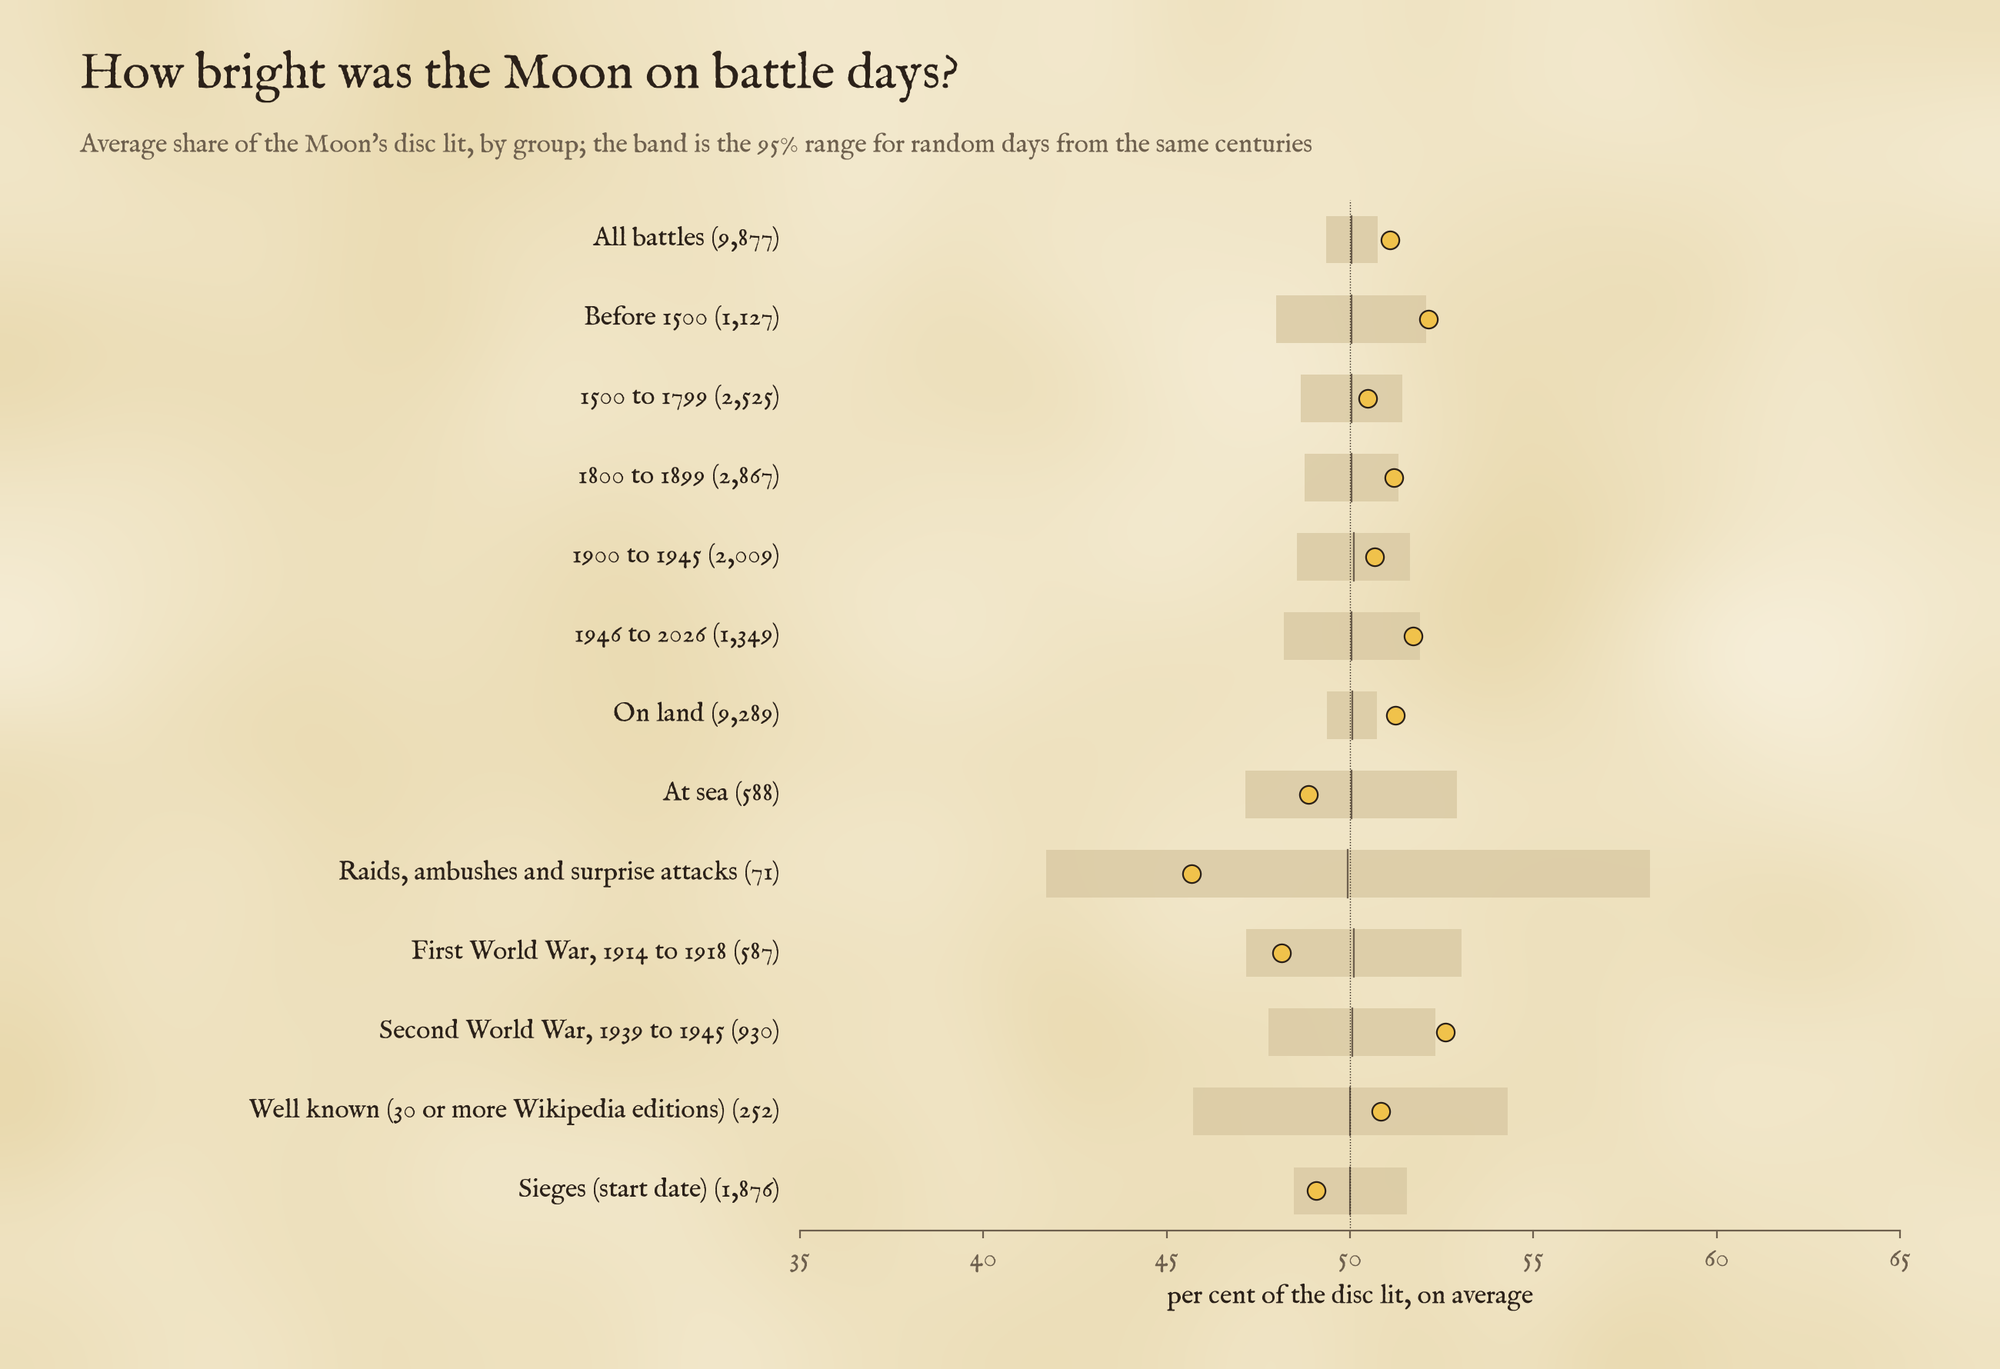
\includegraphics[width=0.92\textwidth]{f_groups.png}
\caption{Mean illuminated fraction on battle days by group, with the 95\% range for random days.}\label{fig:groups}\end{figure}

\subsection{The night before}
On the night before the average battle there were 10.19 hours of darkness, of which the Moon was up for 5.19, against 5.08 on season-matched random nights (difference 0.11 h, standard error 0.04; moonlit share 51.0\% against 49.9\%). The Moon was up at sunrise before 49.9\% of battles and on 49.9\% of random mornings (Figure~\ref{fig:night}).

\begin{figure}[tbp]\centering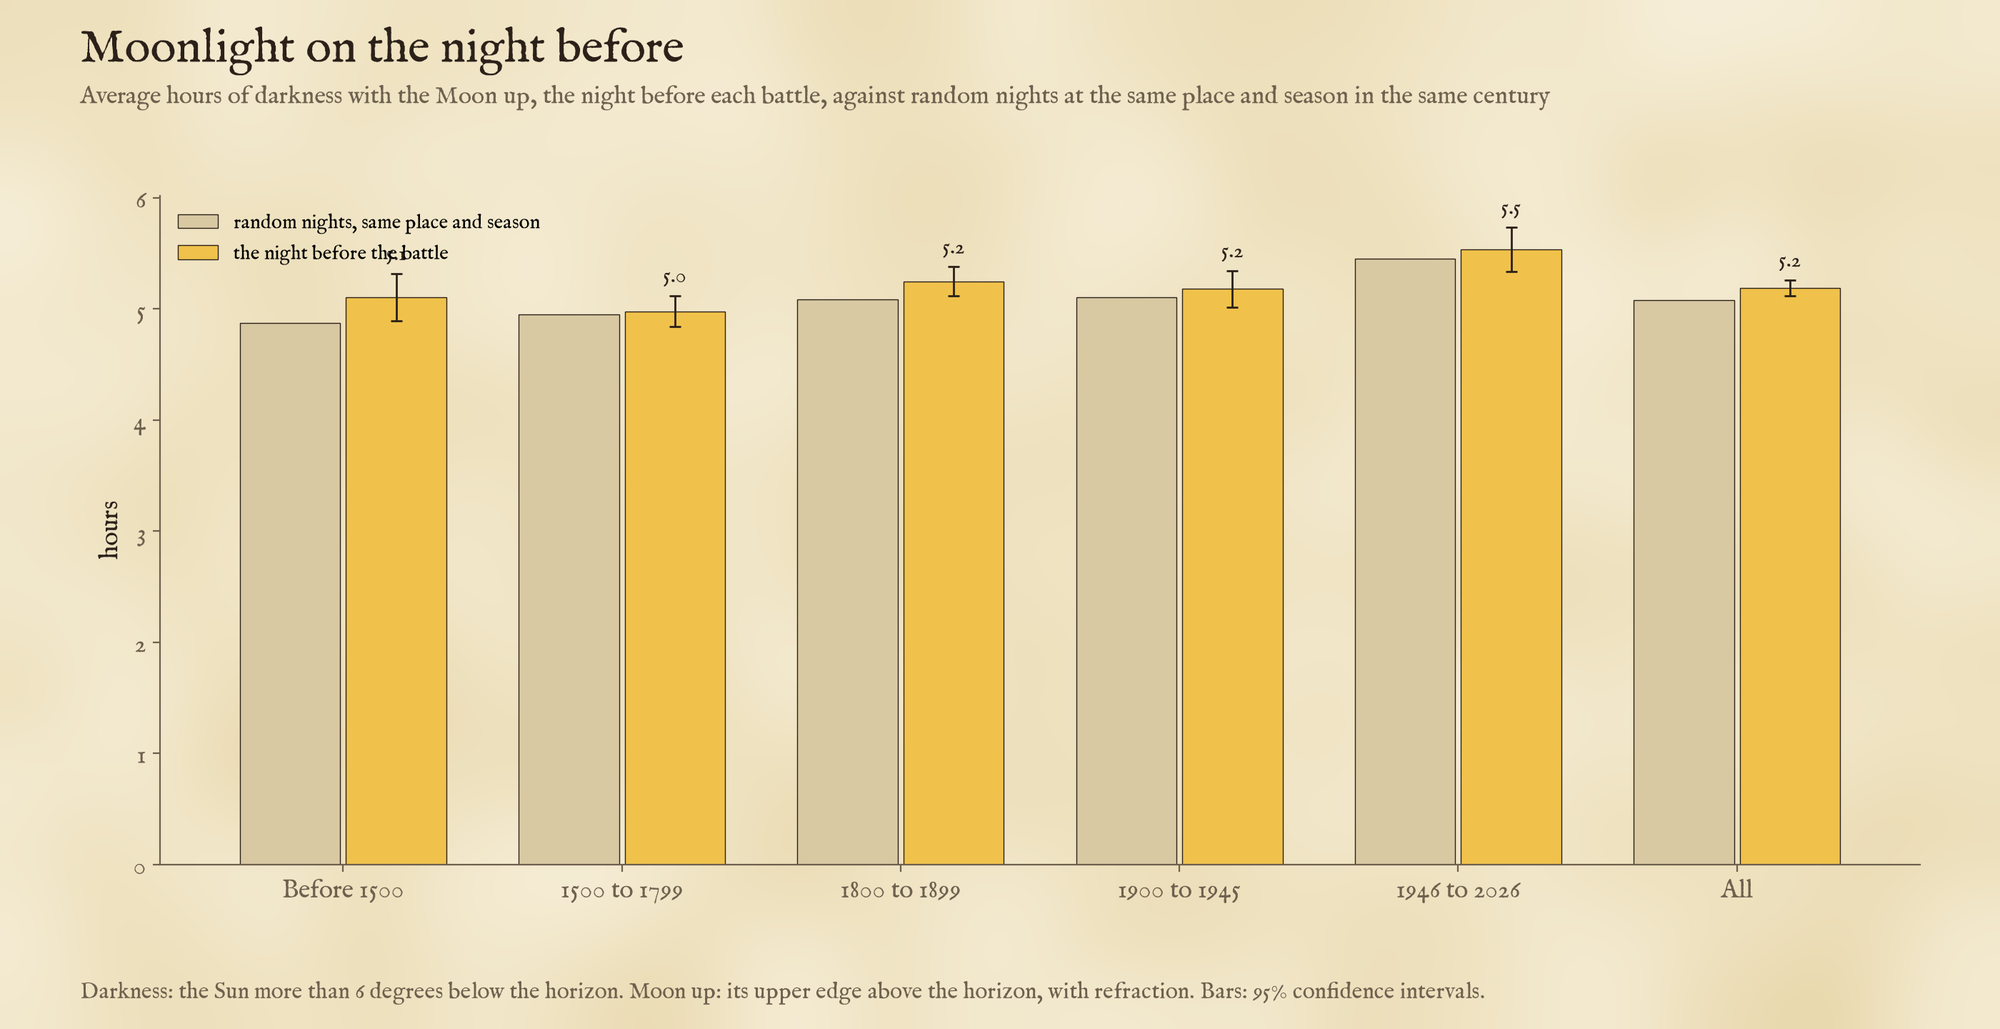
\includegraphics[width=\textwidth]{f_night.png}
\caption{Hours of darkness with the Moon up on the night before battles and on season-matched random nights.}\label{fig:night}\end{figure}

\subsection{Famous battles}
Table~\ref{tab:famous} and Figure~\ref{fig:famous} list the Moon over well-known battles. The calculations agree with what the sources record about the Moon itself: a lunar eclipse on the eve of Pydna \citep{livy} requires a full Moon (calculated: 0.7 days from full); a solar eclipse at the Halys \citep{herodotus,stephenson1997} requires a new Moon (calculated phase 357.5\textdegree); the partial solar eclipse during the battle of Isandlwana in 1879 \citep{espenak} likewise (phase 359.0\textdegree); Badr, on 17 Ramadan in a calendar whose months begin with the new crescent, falls 1.5 days after full. D-Day falls -0.3 days from full Moon and Second El Alamein -0.8; Hastings and Agincourt fell at last quarter, the first day of the Somme, Trafalgar and Naseby at new Moon.

\begin{table}[tbp]\centering\footnotesize\caption{The Moon over famous battles: Gregorian date, phase angle from astronomy-engine and PyEphem, illuminated share (\%), days from the nearest full Moon, and hours of darkness with the Moon up on the night before (of the hours of darkness).}\label{tab:famous}\begin{tabular}{llrrrrr}\toprule Battle & Date & AE & PyEphem & Lit & Full & Moonlit/dark\\\midrule
Halys, 585 BC & 22 May 585 BC & 357.5 & 357.2 & 0 & +14.8 & 0.0/8.2\\
Gaugamela, 331 BC & 26 September 331 BC & 312.1 & 311.9 & 17 & +10.6 & 3.7/11.0\\
Pydna, 168 BC & 19 June 168 BC & 187.6 & 187.4 & 100 & +0.7 & 7.7/7.7\\
Badr, 624 & 15 March 624 & 199.2 & 199.2 & 97 & +1.5 & 11.0/11.2\\
Hastings, 1066 & 20 October 1066 & 272.5 & 272.4 & 48 & +8.3 & 7.7/12.3\\
Crécy, 1346 & 3 September 1346 & 112.3 & 112.2 & 69 & -6.2 & 4.0/9.2\\
Kosovo, 1389 & 23 June 1389 & 247.3 & 247.3 & 69 & +6.0 & 4.5/7.5\\
Agincourt, 1415 & 3 November 1415 & 275.5 & 275.5 & 45 & +7.1 & 7.5/13.0\\
Bosworth, 1485 & 31 August 1485 & 135.9 & 135.9 & 86 & -3.4 & 4.3/8.8\\
La Noche Triste, 1520 & 10 July 1520 & 179.9 & 179.9 & 100 & -0.0 & 9.0/9.0\\
Lepanto, 1571 & 17 October 1571 & 230.5 & 230.5 & 82 & +4.2 & 10.0/11.8\\
Naseby, 1645 & 24 June 1645 & 10.4 & 10.4 & 1 & -14.5 & 0.0/5.3\\
Culloden, 1746 & 27 April 1746 & 75.1 & 75.1 & 37 & -7.9 & 6.0/7.0\\
Trafalgar, 1805 & 21 October 1805 & 347.4 & 347.4 & 1 & +12.9 & 0.7/12.0\\
Waterloo, 1815 & 18 June 1815 & 142.0 & 142.0 & 89 & -3.3 & 5.0/5.8\\
Gettysburg, 1863 & 1 July 1863 & 186.2 & 186.2 & 100 & +0.4 & 7.8/7.8\\
Isandlwana, 1879 & 22 January 1879 & 359.0 & 359.0 & 0 & +13.9 & 0.0/9.5\\
The Somme, 1916 & 1 July 1916 & 11.3 & 11.3 & 1 & -13.7 & 0.0/6.0\\
Battle of Britain, 1940 & 10 July 1940 & 66.6 & 66.6 & 30 & -8.9 & 0.8/5.3\\
Pearl Harbor, 1941 & 7 December 1941 & 225.0 & 225.0 & 85 & +4.1 & 9.8/12.2\\
Stalingrad, 1942 & 23 August 1942 & 142.4 & 142.4 & 90 & -2.8 & 5.8/8.7\\
Second El Alamein, 1942 & 23 October 1942 & 171.1 & 171.1 & 99 & -0.8 & 11.5/12.0\\
D-Day, 1944 & 6 June 1944 & 176.4 & 176.4 & 100 & -0.3 & 6.3/6.3\\
\bottomrule\end{tabular}\end{table}

\begin{figure}[tbp]\centering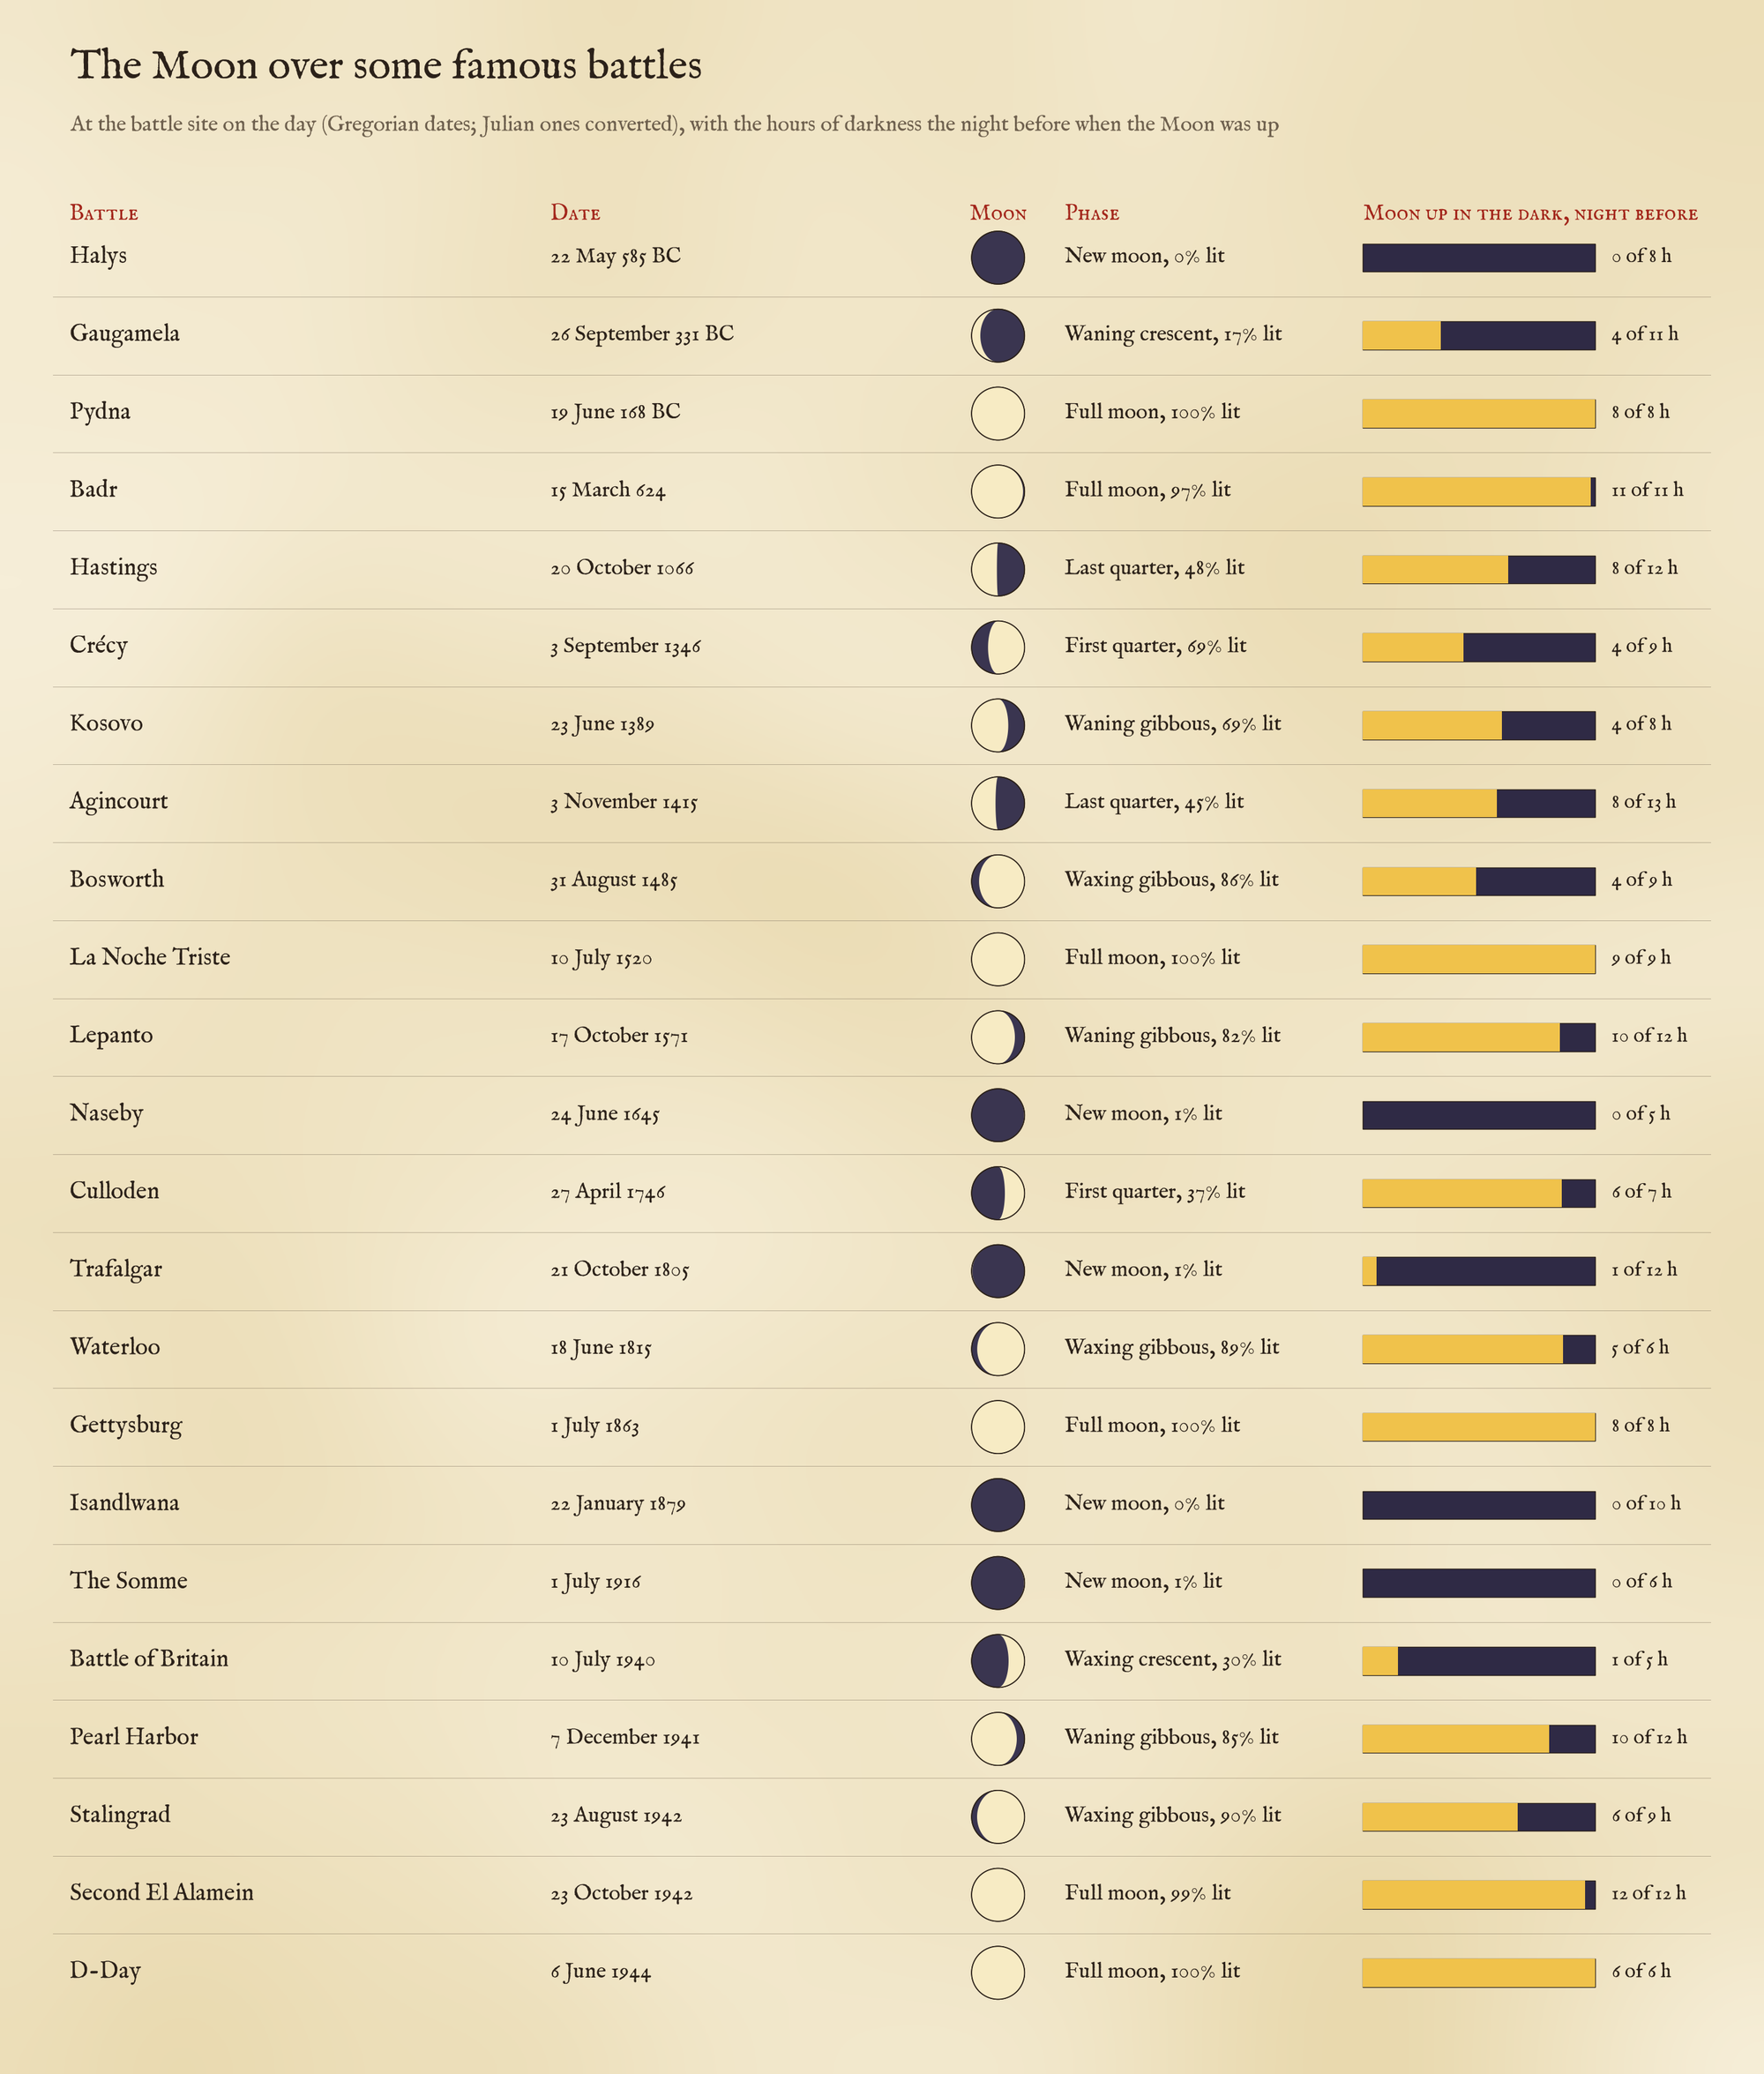
\includegraphics[width=0.9\textwidth]{f_famous.png}
\caption{The Moon over famous battles.}\label{fig:famous}\end{figure}

\begin{figure}[tbp]\centering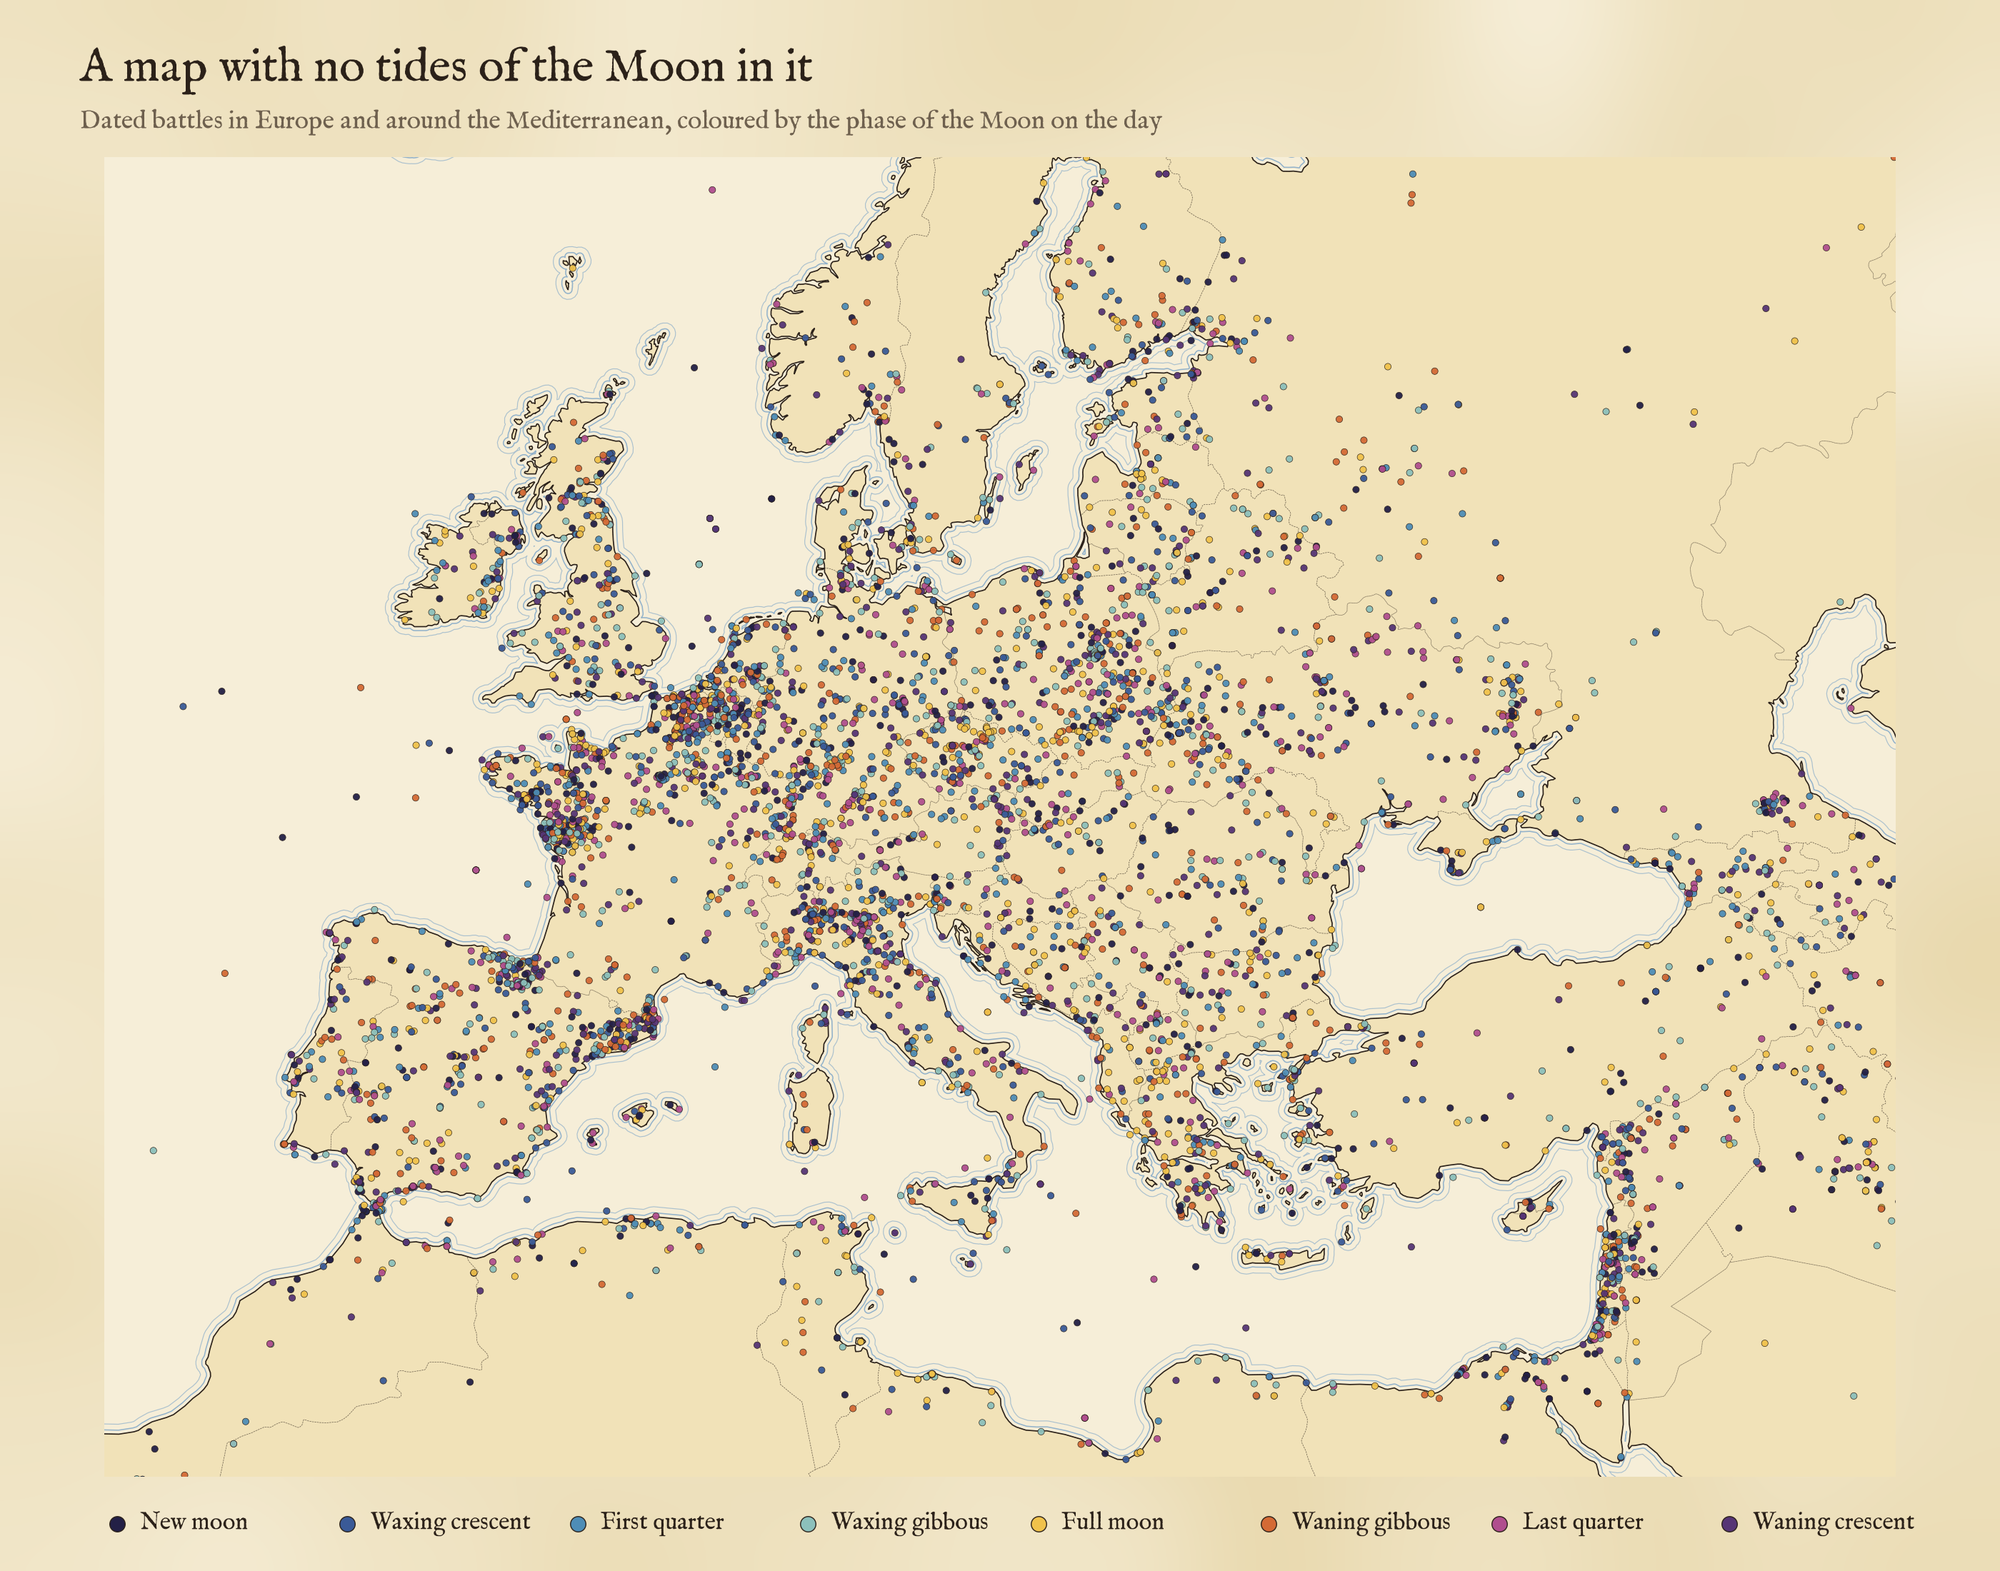
\includegraphics[width=\textwidth]{f_map.png}
\caption{Dated battles in Europe and the Mediterranean by phase of the Moon.}\label{fig:map}\end{figure}

\begin{figure}[tbp]\centering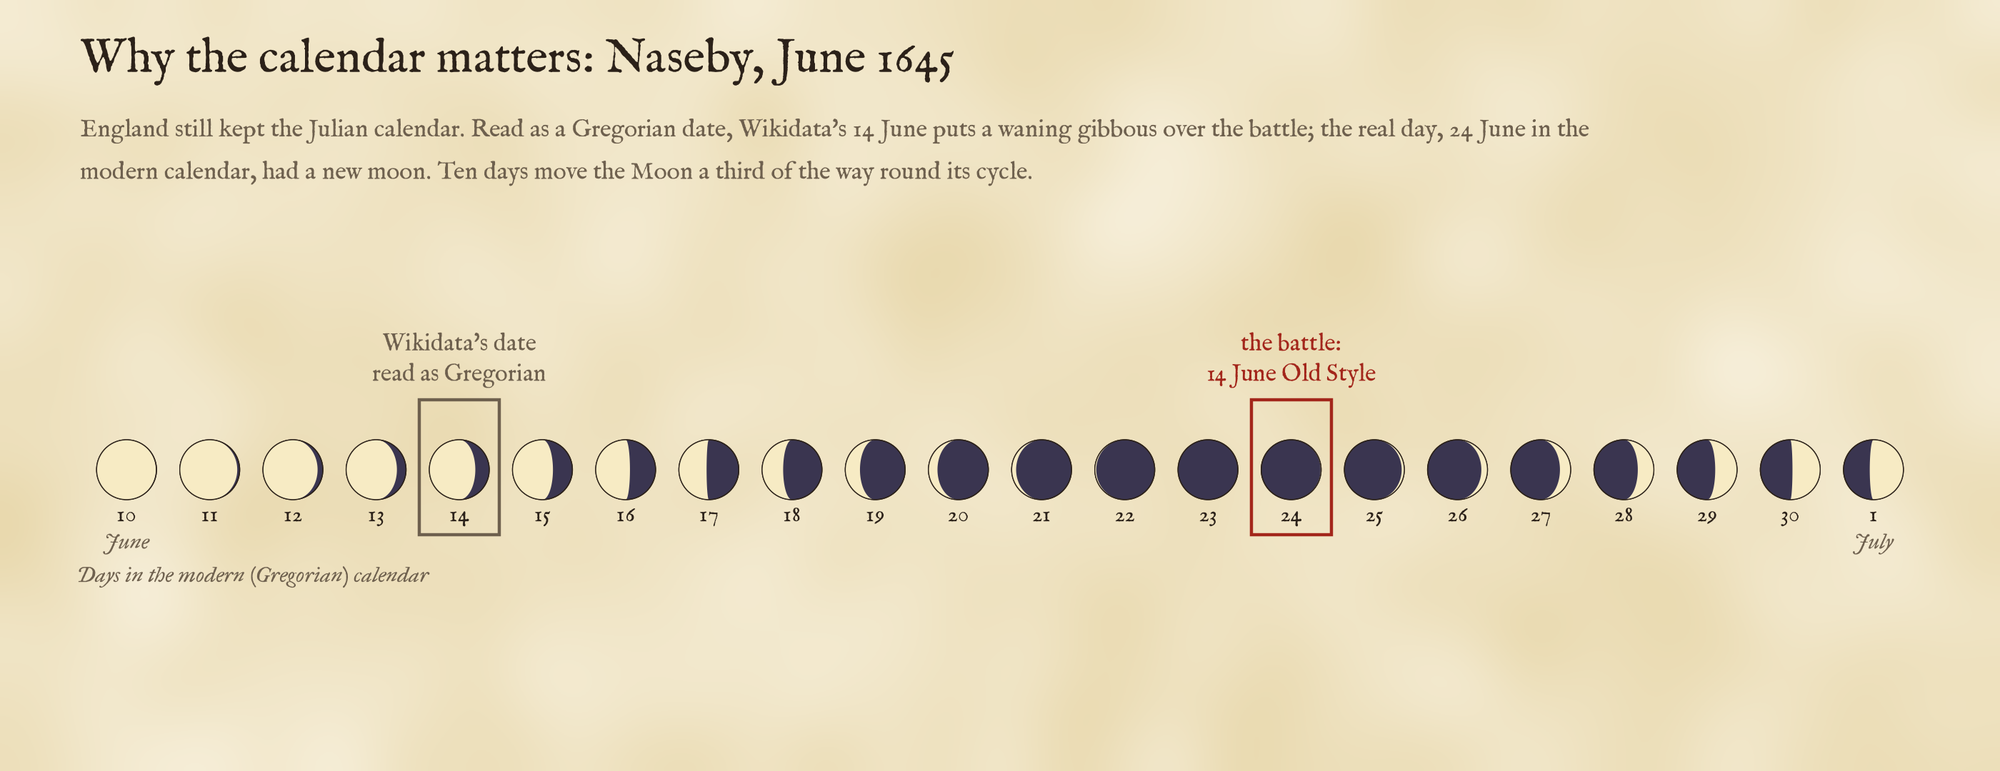
\includegraphics[width=\textwidth]{f_calendar.png}
\caption{The Moon from 10 June to 1 July 1645: Naseby's Old Style date read as Gregorian, and the real day.}\label{fig:cal}\end{figure}

\section{Limitations}
Wikidata's coverage is uneven: 63\% of tested battles are from 1800 or later, and Europe dominates (Figure~\ref{fig:map}). Battle dates are the recorded first day, not the hour fighting began, and some items are multi-day operations or campaigns. Sub-battles of the same day are not independent, which is why the per-date sensitivity matters. Calendar errors certainly remain outside the cases checked, for example Russian Old Style dates before 1918 entered as Gregorian, and dates in Islamic or other lunar calendars, which fix the phase by construction. Such errors move a battle's Moon at random and so dilute any real pattern rather than create one; a strong lunar rhythm would survive them, a weak one would not. The analysis says nothing about the many decisions in which the Moon was weighed but did not decide the date.

\section{Data availability}
The interactive map is at \url{https://maps.tristanhotham.com/battle-moons/}; data and code at \url{https://github.com/Tristan-Hotham/battle-moons}. \texttt{battles.csv} gives every item with its settled date, calendar rule, phase and the night before; \texttt{calendar\_checks.csv} and \texttt{famous.csv} the hand checks; \texttt{results.json} every number in this paper. Wikidata is CC0 and so is the derived data; text and figures CC BY 4.0; code MIT.

\section*{AI assistance}
I wrote the text, with drafting and editing assistance from Claude (Anthropic), which also helped prepare the analysis code. I reviewed and checked all text and results.

\begin{thebibliography}{9}
\bibitem[Bast and Buchhold(2017)]{qlever} Bast, H. and Buchhold, B. (2017) QLever: a query engine for efficient SPARQL+Text search. \textit{Proceedings of the 2017 ACM Conference on Information and Knowledge Management (CIKM)}, 647-656.
\bibitem[Cross(2026)]{astronomyengine} Cross, D. (2026) Astronomy Engine: astronomy calculation library. Software, MIT licence. \url{https://github.com/cosinekitty/astronomy}
\bibitem[Espenak and Meeus(2006)]{espenak} Espenak, F. and Meeus, J. (2006) \textit{Five Millennium Canon of Solar Eclipses: $-$1999 to +3000}. NASA Technical Publication TP-2006-214141.
\bibitem[Fisher(1993)]{fisher1993} Fisher, N. I. (1993) \textit{Statistical Analysis of Circular Data}. Cambridge University Press.
\bibitem[Herodotus(c. 430 BC)]{herodotus} Herodotus, \textit{Histories}, 1.74.
\bibitem[Livy(c. 10 BC)]{livy} Livy, \textit{Ab Urbe Condita}, 44.37.
\bibitem[Meeus(1998)]{meeus} Meeus, J. (1998) \textit{Astronomical Algorithms}, second edition. Willmann-Bell.
\bibitem[Reingold and Dershowitz(2018)]{reingold} Reingold, E. M. and Dershowitz, N. (2018) \textit{Calendrical Calculations: The Ultimate Edition}. Cambridge University Press.
\bibitem[Rhodes(2026)]{pyephem} Rhodes, B. (2026) PyEphem: astronomical computations for Python. Software. \url{https://rhodesmill.org/pyephem/}
\bibitem[Stephenson(1997)]{stephenson1997} Stephenson, F. R. (1997) \textit{Historical Eclipses and Earth's Rotation}. Cambridge University Press.
\bibitem[Vrande\v{c}i\'{c} and Kr\"{o}tzsch(2014)]{wikidata} Vrande\v{c}i\'{c}, D. and Kr\"{o}tzsch, M. (2014) Wikidata: a free collaborative knowledgebase. \textit{Communications of the ACM} 57(10), 78-85.
\end{thebibliography}
\end{document}
